\chapter{Results \& Evaluation} \label{Evaluation}

Here, we will discuss how the implementations of the algorithms in our scenario were tested and ensured that they ran as they should.

\section{Software Testing}

Due to the nature of the project (being several implementations of a computer game), the testing behind this project has solely revolved around trial-and-error, messing around with the exported variables in the Godot editor to see how things worked and what configurations worked best for our scenario. This involved taking many screenshots of generated levels and examining things by eye, seeing how layouts compared across implementations.

Despite this, it was eventually decided to run some simple performance tests to see how long each algorithm ran. These tests took some of the custom export variables from the scene scripts and ran them several times, with an average time calculated to the nearest millisecond. The results of these tests are all in table in the \hyperref[Appendix]{Appendix}.

\section{Comparing the Different Algorithms and Drawing Conclusions on Which Ones Are Best}

\subsection{Performance}

With the L-System implementation, there were no problems whatsoever running the game very quickly on the author of this report's machine, and quickly got satisfactory results. The table in Figure \ref{fig:table3} shows that the processing times remained miniscule, even as the length of the axiom increased.

While the Noise implementation was slower than the L-System implementation by a magnitude, it was still satisfactorily quick. Some timed tests were run in which this paper's author tested how some of the properties affected the time it took to generate the noise. These tests are referred to in tables \ref{fig:table1}, in which each noise algorithm was paired with each cellular distance function, and \ref{fig:table2}, in which each noise algorithm was paired with each fractal type. With the default values set \hyperref[noisedefaults]{here}, it was found that it took an average of 81ms, as shown in table \ref{fig:table6}.

With Poisson Disk Sampling, the higher the number of rejection samples (that is, the higher the maximum number of times a cell was sampled before it was either accepted or ultimately rejected), the longer it took to generate a complete level layout, and even, due to the nature of the tile map compared to the algorithm's \textit{usual} use (of scattering dots on a plane), it was not maximal (not all points had cells painted for them; some cells had their tiles overwritten as well). Using 8 rejection samples was usually enough to yield a satisfactory level layout while also keeping level creation times to a satisfactory minimum. It took an average of 268ms to work satisfactory with 8 rejection samples in the tests in table \ref{fig:table4}. If the rejection samples were given a too high value, there was a high  chance that the game would hang and not return any cell points at all, because it just took \textit{way} too long to process.

Voronoï Cells took the longest to compute on average. Computations with the Euclidean distance measurement took longer than those measured with the Manhattan distance.

\subsection{Layouts}

Of the 4 implementations that were made for this project, the Noise and Poisson Disk Sampling implementation were by far the most similar, followed by the L-System implementation, and then the Voronoï Cells implementation, which was far and away the most unique.

While the noise implementations varied greatly depending on what settings were used, and the way the implementation was designed allowed for very many possibilities as to how the noise would turn out (and how it would affect the final level), the results that were returned produced the most similar results to that of the Poisson Disk Sampling implementation had the following configurations:

\begin{itemize} \label{noisedefaults}
    \item Noise Type (``noise\_type"): Simplex Smooth
    \item Fractal Type (``fractal\_type"): Fractal None
    \item Cellular Distance Type/Function (``cellular\_distance\_type"): Distance Euclidean
    \item Noise Frequency (``noise\_frequency"): 0.894
    \item Tree Cap (``tree\_cap"): -0.048
    \item Building Cap (``building\_cap"): -0.252
    \item Building Overtakes Tree (``building\_overtakes\_tree"): 0.12
\end{itemize}

The default noise frequency in ``FastNoiseLite" is 0.01, which results in smoother and less disparate noise. As seen in Figure \ref{fig:simplexsmooth0.01}, the smoother noise and lower frequency results in a distinct kind of level layout in which represents some of the noise values in the image very clearly, such that tiles (both buildings and trees) are bunched together in partially interconnected groups, forming long, large lines of painted tiles. To describe this as best as possible, it is easy to discern that the level layout was determined from a noise image. Using a higher noise frequency to produce rougher noise, and more disparate level layouts, yields results like in Figure \ref{fig:simplexsmoothdefault1}, which makes it very similar to the layouts yielded in the Poisson Disk Sampling implementation and, to a lesser extent, the L-System implementation. While the author of this report's personal tastes are fond of the former kind of level layout, part of the aim of this project was to compare in terms of which could produce the most similar, and, compared to the L-System and Poisson Disk Sampling implementations, the Noise implementation with the frequency set to 0.01 was far too distinct, hence the want to change it up.

\begin{figure}[H]
    \centering
    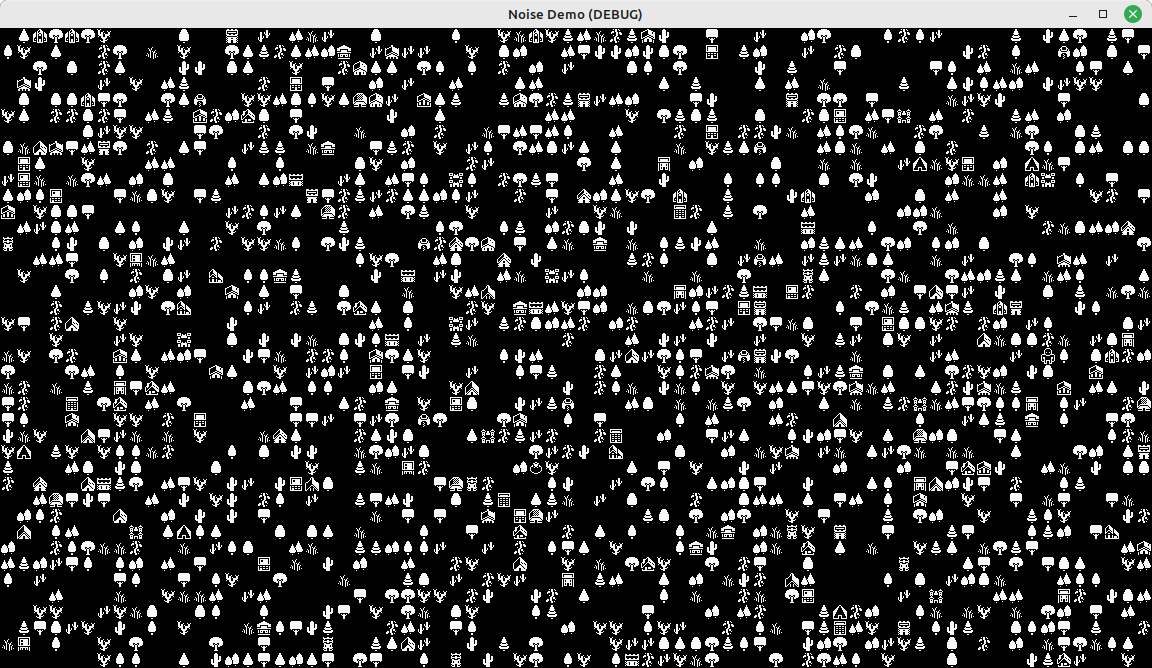
\includegraphics[width=\textwidth]{Images/simplex_smooth_default_1.png}
    \caption{A level of our scenario generated in the Simplex Noise implementation, using all of the default values \hyperref[noisedefaults]{shown here}. The level took a total of 99 milliseconds to be made.}
    \label{fig:simplexsmoothdefault1}
\end{figure}

\begin{figure}[H]
    \centering
    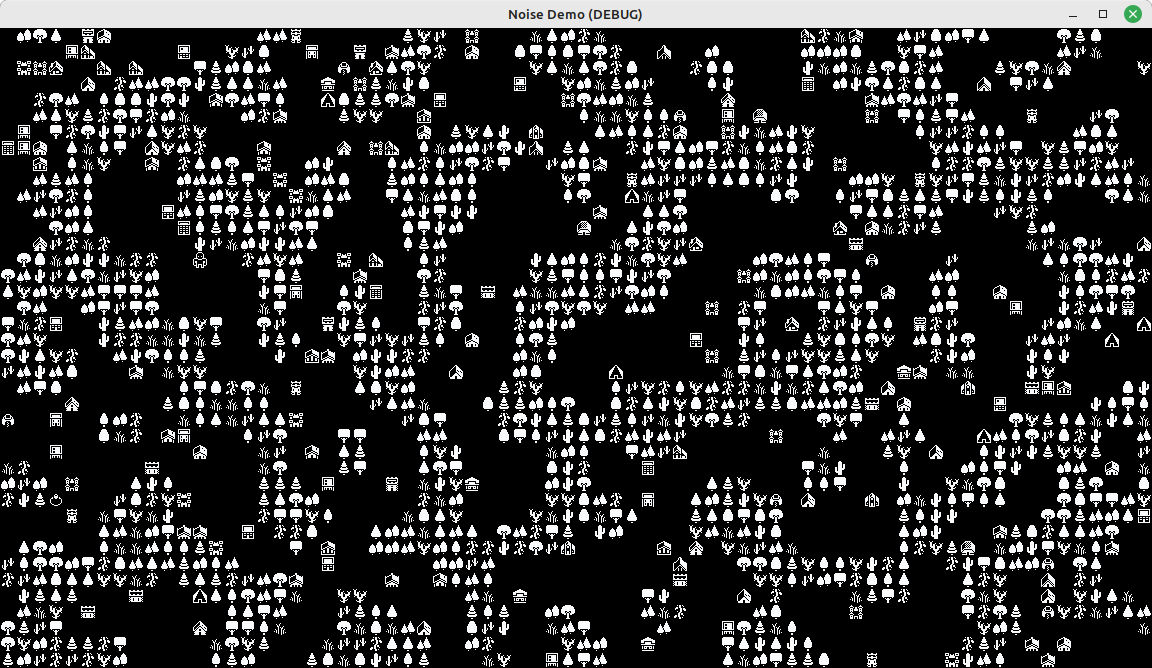
\includegraphics[width=\textwidth]{Images/simplex_smooth_0.01_frequency.png}
    \caption{A level of our scenario generated in the Simplex Noise implementation, setting the noise frequency to 0.01 (the default value for noise frequency in ``FastNoiseLite") and using the rest of the defaults \hyperref[noisedefaults]{shown here}. The level took a total of 104 milliseconds to be made.}
    \label{fig:simplexsmooth0.01}
\end{figure}

The 